La identificación de partículas es parte del proceso de análisis y estudio en el \LHC, para hacer eficiente el proceso de detección, algoritmos y nuevos conceptos tuvieron que definidos e implementados para un aprovechamiento del equipamiento, con la intención de maximizar las observaciones válidas de las partículas que se estudian, en especial la identificación de procesos en los que intervienen los muones sigue siendo uno de los objetivos del proyecto por lo que se hace necesario analizar parte del proceso de identificación y reconstrucción de muones.

\subsubsection{Reconstrucción de muones.}
La reconstrucción de muones es un algoritmo sistémico que se ejecuta en un software de reconstrucción que utiliza información de impacto para rechazar objetos físicos, muones. La reconstrucción de muones se realiza en el rastreador de silicio y el sistema de muones, y se compone de tres pasos secuenciales: reconstrucción local, reconstrucción independiente y reconstrucción global. 

La reconstrucción local utiliza la información del golpe recopilada por el sistema muon para construir pistas; entonces, la información de la pista, como entrada, se alimenta al algoritmo de reconstrucción independiente. La reconstrucción global utiliza no solo información de reconstrucción independiente, sino también golpes de seguimiento de silicio. La reconstrucción del muón coincide con el camino del muón desde el sistema de muones al rastreador de silicio. La reconstrucción independiente se llama reconstrucción de Level-2 y la reconstrucción global se llama reconstrucción de Level-3. Los muones reconstruidos por reconstrucción independiente y global se denominan, respectivamente, muones independientes y muones globales.

\begin{figure}[h!]
\centering
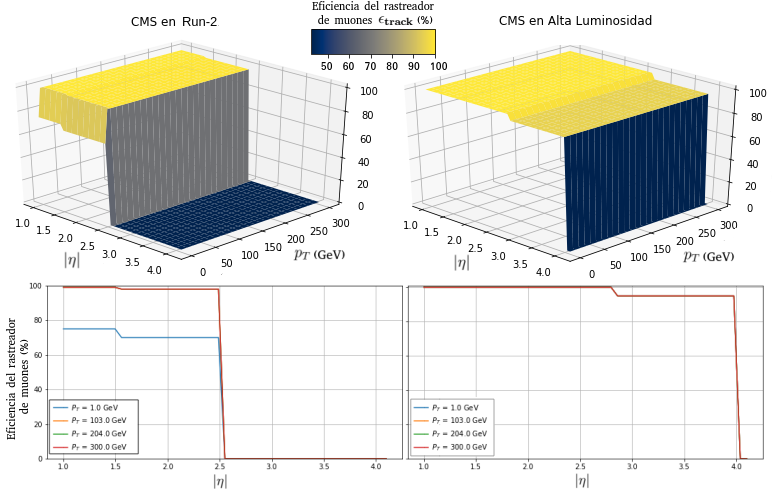
\includegraphics[width=.9\textwidth]{Analisis_y_Resultados/imagenes/Tracking_of_Muon.png}
\caption{Probabilidad de localización de los muones en condiciones de Run-2 y HL.}
\label{Compara_track_muon}
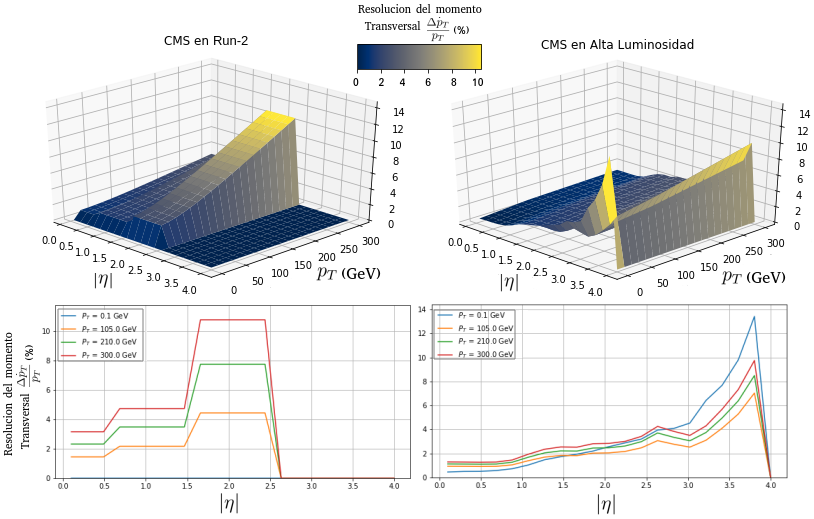
\includegraphics[width=.9\textwidth]{Analisis_y_Resultados/imagenes/Momentum_resolution_of_Muon.png}
\caption{Resolución del momento de los muones en condiciones de Run-2 y HL.}
\label{Compara_sol_muon}
\end{figure}
En la Fig. \ref{Compara_track_muon} se puede observar como aumenta la capacidad del experimento \CMS ~ para diferentes condiciones del experimento, en esta se evidencia el aumento de la detección de los muones con valores de $\eta > 2.4$, esto es parte del proceso de actualización a Alta Luminosidad. Además la resolución de los valores de momento reconstruidos de los muones en las condiciones actuales del experimento y en las previstas de alta luminosidad se puede ver en la Fig. \ref{Compara_sol_muon}, es clara la disminución del error para la región común ($0<\eta < 2.4$).

\subsubsection{Identificación de muones.}

La ``D0 muon ID'' es un algoritmo utilizado para seleccionar candidatos a muones y es un algoritmo complementario para la reconstrucción estándar. A diferencia de la reconstrucción estándar, utiliza información de energía adicional de \textbf{ECAL} y \textbf{HCAL}, y está al revés en términos de información del detector. Muon Identification primero reconstruye las pistas de los rastreadores de silicio y luego utiliza la información de la \textbf{ECAL} y la \textbf{HCAL}.

También se consideran los rastreadores que no están asociados con ningún rastro de muones independiente, lo que le permite reconstruir algunos muones de $p_T$ bajos sin suficiente energía para alcanzar el sistema muónico. Estos bajos p T muones pueden no ser reconstruidos como muones globales, pero son identificados por el algoritmo de identificación de muones. Los muones reconstruidos por el algoritmo de identificación se denominan muones rastreados (``tracker muons'').

\subsubsection{Aislamiento de muones.}

Los muones producidos a partir de objetos pesados como $Z$ y $W$ deben aislarse de los muones producidos a partir del decaimiento $b$ o $c$, el aislamiento de muones (``muon isolation'') tiene como objetivo separar estos diferentes muones, lograndose esta separación calculando la energía transversal total $E_T$ depositada en un calorímetro dentro de un cono a lo largo de la dirección del muón.

\subsubsection{Eficiencia Muon.}

Las secciones anteriores describen brevemente cada parte del experimento \CMS ~ desde la vía interna, más cercana a la línea del haz, hasta el sistema de muones más externo. Muchos análisis físicos requieren la probabilidad de que un muón se reconstruya como un objeto muón, dado que el muón se produce en un evento. En general, esa probabilidad se llama eficiencia. La eficiencia es la relación entre el número de muones que pasan los criterios deseados y el número total de muones producidos, también puede definirse como:
\begin{equation}
\epsilon_\mu = \epsilon_{track} \cdot \epsilon_{id} \cdot 
\epsilon_{iso} \cdot  \epsilon_{trig}
\end{equation}
donde $\epsilon_{track}$ es la eficiencia del rastreador muón, es decir, la probabilidad de que un muón producido en un evento también se reconstruya como un rastreador de silicio, rastreador muón. $\epsilon_{id}$ es la eficiencia de identificación del muón, la probabilidad de que un muón pase por un grupo de criterios de selección, dado que es un muón reconstruido. $\epsilon_{iso}$ es la eficiencia de aislamiento del muón, la probabilidad de que un muón reconstruido esté aislado. $\epsilon_{trig}$ es la eficiencia del disparador, la probabilidad de que un muón reconstruido y aislado se dispare en términos de un umbral de $p_T$ dado.

La eficiencia del muón depende de dos factores principales: la estructura del \CMS ~ y el momento transversal $p_T$ de los muones. La eficiencia del muón está influenciada por la ruta a través de la cual pasa un detector, porque el detector no es homogéneo, por lo tanto, la pseudoapidez $|\eta|$ y el ángulo azimutal $\varphi$ desempeñan un papel en la decisión de la eficiencia del muón. Como el detector es muy simétrico con respecto a $\varphi$ no influye significativamente en la eficiencia del muón. La $p_T$ de los muones decide si tienen suficiente energía para llegar al sistema muónico, debido a que los muones independientes necesitan más de una estación para ser alcanzados en el sistema muónico, los muones con bajo $p_T$ no pueden reconstruirse como muones independientes. Toda esta información es resumida en los paquetes $*.tcl$ de Delphes, aunque solo de forma básica ya que se busca descripción general del sistema.

\begin{figure}[ht]
\centering
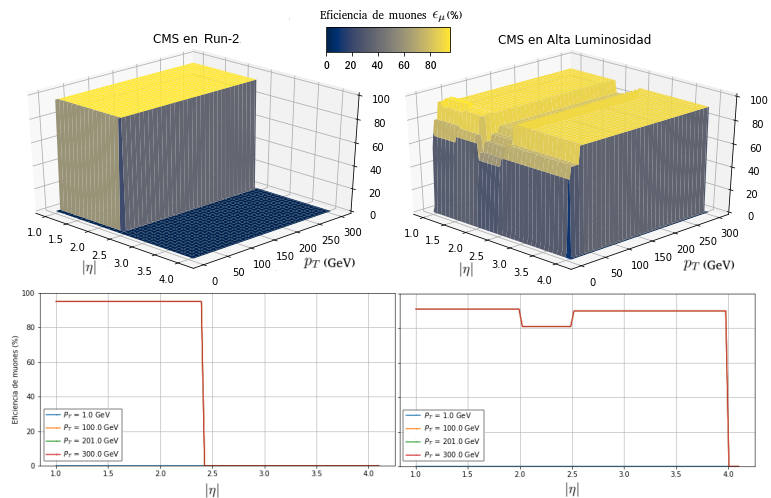
\includegraphics[width=1\textwidth]{Analisis_y_Resultados/imagenes/Eficiencia_of_Muon.png}
\caption{Eficiencia de reconstrucción de los muones en condiciones de Run-2 y HL.}
\label{Compara_eficiencia_muon}
\end{figure}

Como se puede observar en la Fig. \ref{Compara_eficiencia_muon} se extiende como es esperado la eficiencia para valores de $\eta > 2.4$ en la configuración de Alta Luminosidad, esto como resultado de la actualización pĺanificada por el proyecto.






